\section{Analysis}\label{sec:analysis}

\comment{Present datasets???}

%$\datasetA = \big\{ (\vec{x}^{(1)}, y^{(1)}), \,  (\vec{x}^{(2)}, y^{(2)}), \,\dots, \, (\vec{x}^{({\npointsA})}, y^{(\npointsA)}) \big\}$ 

\comment{Maybe write something about the codes?}


OUTLINE:
\begin{enumerate}
    \item Gradient descent \begin{enumerate}
        \item[-] OLS and Ridge on regression problem
    \end{enumerate}
    \item Building our FFNN
    \item Regression problem \begin{enumerate}
        \item[-] try different activation functions
    \end{enumerate}
    \item Classification problem \begin{enumerate}
        \item[-] compare with logistic regression 
    \end{enumerate}
\end{enumerate}

\subsection{Gradient descent}\label{sec:analysis_SGD}

    We write a code that  \fillertext


    Using the SGD method, we perform an OLS regression on a dataset generated by a third order polynomial with some added noise,
    \begin{equation}
        f(x) = 2.0x + 1.7x^2 -0.40x^3 \, +\, 0.10\mathcal{N}(0, 1),
    \end{equation}
    and we consider $n=400$ datapoints. In particular, we aim to minimise the cost function in eq. \eqref{eq:linear_regression_cost_function} with $\lambda=0$ for which we need to tune the learning rate $\eta$. We perform the same analysis using the Ridge cost function, i.e. $\lambda > 0$ in eq. \eqref{eq:linear_regression_cost_function}, but here we need to tune the penalty parameter $\lambda$ as well as the learning rate $\eta$. 

    We do not present many figures to describe this part of the analysis. We justify this by arguing that the purpose of this part is to test the SGD code, and then by extension the GD code, and give an idea of the effect of changing optimisers. 

    In figure \ref{fig:simple_reg_errors_ridge}  \fillertext

    \begin{figure}
        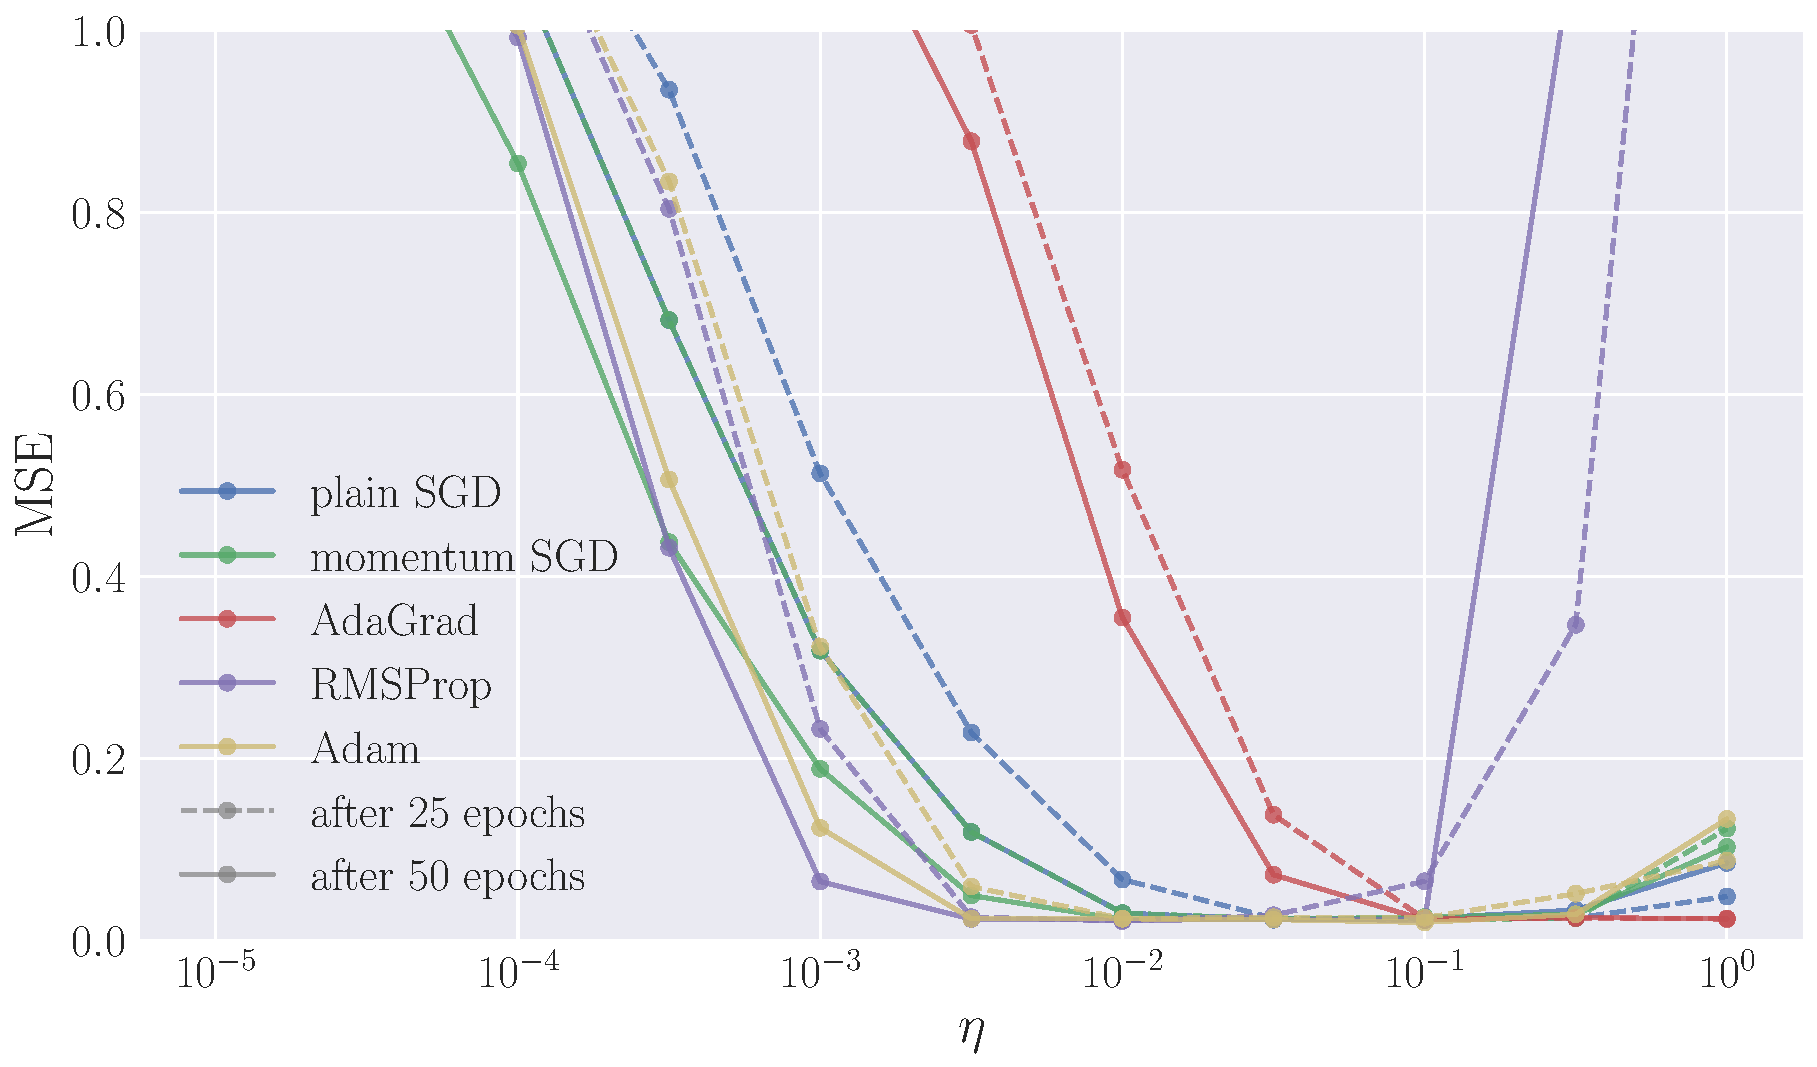
\includegraphics[width=\linewidth]{ridge_errors_gradient_descent.pdf}
        \caption{The graphs show how the test MSE evolves as the global learning rate $\eta$ increases for different update rules in the SGD algorithm. The penalty parameter is $\lambda=0.1$, and we have used $m=40$ minibatches. $\gamma=0.5$ for the momentum SGD and the other relevant hyperparameters are set to their defaults in accordance with section \ref{sec:tuning}. The dashed graphs show the MSE after 25 iterations and the solid graphs represent the MSE after 25 additional iterations. All solvers were initilised by the same random vector $\svec{\theta}_0$.}
        \label{fig:simple_reg_errors_ridge}
    \end{figure}

    We will study more thoroughly the dependencies on the number of epochs, the number of minibatches ($m$) and the penalty parameter ($\lambda$) in the NN analysis of the Franke function in section \ref{sec:analysis_NN}. 




    
\subsection{Neural network}\label{sec:analysis_NN}
    We will build our FFNN (\ref{item:prepocess}-\ref{item:optimiser}) and solve a supervised learning problem (\ref{item:train}-\ref{item:review}) using the steps listed below \citep{mhjensen}.

    \begin{enumerate}[label=(\roman*)]
        \item\label{item:prepocess} Collect and prepocess data, that is we extract 80\% of the dataset and reserve the rest for validation. The data is then scaled using standard score normalisation\footnote{Formula found in \cite{mhjensen}, or page 6 of the \projectOne-report.} with respect to the training data.
        \item\label{item:architecture} Define the model and design its architecture. In practice, this means to decide on hyperparameters of the NN such as depth ($L$) and activation function(s) ($g$).
        \item\label{item:optimiser} Choose loss function and optimiser. For regression we will use the MSE score \eqref{eq:linear_regression_cost_function} as the estimator of loss, whereas the classification problem estimates the loss according to the cross entropy \eqref{eq:logistic_regression_cost_function}. We will use SGD as optimiser, but we have various alternatives for the exact optimisation algorithm (see section \ref{sec:tuning}).
        \item\label{item:train} Train the network to find the right weights and biases.
        \item\label{item:assess} Validate model, i.e. assess model performance by applying it on the test data.
        \item\label{item:review} Adjust hyperparameters, and if necessary review the network architecture. That is to say, if the result is not satisfactory even after tuning the hyperparameters, return to step \ref{item:architecture} and start over from there. 
    \end{enumerate}

    %In practice, the steps \ref{item:architecture}-\ref{item:review} will be performed several times 
    

\subsection{Regression problem}\label{sec:analysis_regression}


    Our dataset is once again fictional as it is generated by the Franke function from \projectOne\footnote{Equation (10) in the report.} with an added noise of $0.1 \mathcal{N}(0, 1)$ for a set of coordinates in the plane. We split and standardise the $20\times 20$ datapoints, which concludes step \ref{item:prepocess}. 






\subsection{Classification problem}\label{sec:analysis_classification}



